% Created 2020-06-29 lun 12:39
% Intended LaTeX compiler: pdflatex
\documentclass[presentation,aspectratio=169]{beamer}
\usepackage[utf8]{inputenc}
\usepackage[T1]{fontenc}
\usepackage{graphicx}
\usepackage{grffile}
\usepackage{longtable}
\usepackage{wrapfig}
\usepackage{rotating}
\usepackage[normalem]{ulem}
\usepackage{amsmath}
\usepackage{textcomp}
\usepackage{amssymb}
\usepackage{capt-of}
\usepackage{hyperref}
\usepackage{khpreamble}
\usepackage{amssymb}
\usepgfplotslibrary{groupplots}
\newcommand*{\shift}{\operatorname{q}}
\usetheme{default}
\author{Kjartan Halvorsen}
\date{2020-06-29}
\title{Computerized control - Introduction}
\hypersetup{
 pdfauthor={Kjartan Halvorsen},
 pdftitle={Computerized control - Introduction},
 pdfkeywords={},
 pdfsubject={},
 pdfcreator={Emacs 26.3 (Org mode 9.3.6)}, 
 pdflang={English}}
\begin{document}

\maketitle

\section{Presentation}
\label{sec:org4ef8d77}
\begin{frame}[label={sec:org30ddc64}]{Who am I?}
\end{frame}

\begin{frame}[label={sec:orgdb5b6e2}]{Who are you?}
\end{frame}

\section{Intro}
\label{sec:org07a8e15}
\begin{frame}[label={sec:org73918ef}]{Goal of the course}
To be able to \alert{analyze}, \alert{design}, \alert{implement} and \alert{evaluate} computerized product and process control systems with a focus on practical application.
\end{frame}

\begin{frame}[label={sec:orga523b98}]{Feedback control in continuous time model}
\begin{center}
\includegraphics[width=0.6\linewidth]{../../figures/block1}
\end{center}
\end{frame}

\begin{frame}[label={sec:org330e38c}]{Feedback control in continuous time model}
\begin{center}
\includegraphics[width=0.6\linewidth]{../../figures/block1}
\end{center}

\alert{Activity} Write down three interesting \alert{\alert{properties}} of a control system (write as PM in the chat)
\end{frame}
\begin{frame}[label={sec:org809c51a}]{Feedback control in real system}
\begin{center}
\includegraphics[width=0.7\linewidth]{../../figures/comp-contr-sys.png}
\end{center}
\footnotesize From Åström and Murray \emph{Feedback systems: An introduction for scientists and engineers}
\end{frame}

\begin{frame}[label={sec:orgef9bd9a}]{Feedback control in real system}
\begin{center}
\includegraphics[width=0.7\linewidth]{../../figures/fig7-2.png}
\end{center}
\footnotesize From Åström and Wittenmark \emph{Computer-controlled systems}
\end{frame}

\begin{frame}[label={sec:org293b331}]{Why computerized control?}
\end{frame}

\begin{frame}[label={sec:org8cfacea}]{Computers everywhere}
\begin{center}
\includegraphics[width=0.7\linewidth]{../../figures/electronics-in-cars.png}
\end{center}
\begin{LaTeX}
\{\tiny Winning share in automotive semiconductors. McKinsey report 2013 \} 
\end{LaTeX}
\end{frame}

\begin{frame}[label={sec:org566cfc5}]{Two approaches to designing a  discrete-time controller}
\begin{enumerate}
\item Do design the controller in the continuous-time domain (methods from control engineering class). Then discretize the continuous-time controller.
\includegraphics[width=0.7\linewidth]{../../figures/block1} \(F_d(z) \approx F(s)\)
\item Determine discrete-time model of the plant. Do design in discrete-time domain.
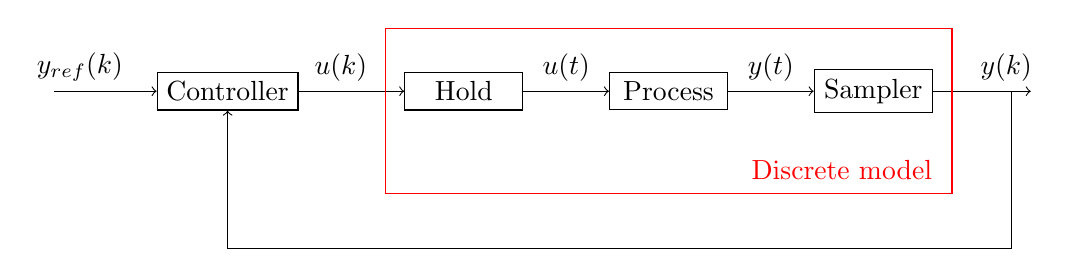
\begin{tikzpicture}[node distance=22mm, block/.style={rectangle, draw, minimum width=15mm}, sumnode/.style={circle, draw, inner sep=2pt}]

  \node[coordinate,] (refinput) {};
  \node[block, right of=refinput] (controller)  {Controller};
  \node[block, right of=controller, node distance=30mm] (zoh)  {Hold};
  \node[block, right of=zoh, node distance=26mm] (plant)  {Process};
  \node[block, right of=plant, node distance=26mm] (sampler)  {Sampler};
  \node[coordinate, right of=sampler, node distance=20mm] (output) {};

  \draw[->] (refinput) -- node[above, near start] {$y_{ref}(k)$} (controller);
  \draw[->] (controller) -- node[above, pos=0.4] {$u(k)$} (zoh);
  \draw[->] (zoh) -- node[above] {$u(t)$} (plant);
  \draw[->] (plant) -- node[above] {$y(t)$} (sampler);
  \draw[->] (sampler) -- node[pos=0.8, coordinate] (measure) {} node[above, near end] {$y(k)$} (output);
  \draw[->] (measure) -- ++(0,-20mm) -| (controller);
  \draw[red] (42mm, -13mm) rectangle (114mm, 8mm);
  \node[red] at (100mm, -10mm) {Discrete model};
\end{tikzpicture}
\end{enumerate}
\end{frame}
\section{Example: Diskdrive arm position control}
\label{sec:org7a0b64a}
\begin{frame}[label={sec:org04d1156}]{Position control of a diskdrive arm}
\begin{columns}
\begin{column}{0.5\columnwidth}
\includegraphics[height=0.5\textheight]{../../figures/diskdrive.png}

\tiny "Laptop-hard-drive-exposed" by Evan-Amos - Own work. Licensed under CC BY-SA 3.0 via Commons
\end{column}
\begin{column}{0.5\columnwidth}
\[ J\ddot{\theta}(t) = u(t) + v(t) \]
\begin{center}
  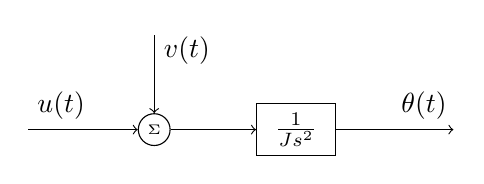
\begin{tikzpicture}[node distance=22mm, block/.style={rectangle, draw, minimum width=10mm}, sumnode/.style={circle, draw, inner sep=2pt}]

    \node[coordinate] (input) {};
    \node[sumnode, right of=input, node distance=16mm] (sum) {\tiny $\Sigma$};
    \node[block, right of=sum, node distance=18mm] (plant)  {$\frac{1}{Js^2}$};
    \node[coordinate, above of=sum, node distance=12mm] (disturbance) {};
    \node[coordinate, right of=plant, node distance=20mm] (output) {};

    \draw[->] (input) -- node[above, pos=0.3] {$u(t)$} (sum);
    \draw[->] (sum) -- node[above] {} (plant);
    \draw[->] (plant) -- node[above, near end] {$\theta(t)$} (output);
    \draw[->] (disturbance) -- node[right, pos=0.2] {$v(t)$} (sum);
  \end{tikzpicture}
\end{center}

\alert{Activity} Write three relevant performance criteria for the closed-loop control system (position servo)!
\end{column}
\end{columns}
\end{frame}

\begin{frame}[label={sec:orgde37a2d}]{Controller design in continuous time}

\begin{center}
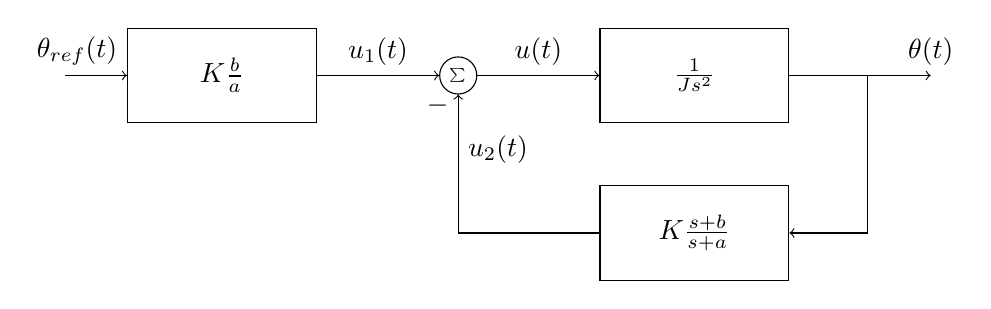
\begin{tikzpicture}
\tikzset{node distance=2cm, 
    block/.style={rectangle, draw, minimum height=12mm, minimum width=24mm},
    sumnode/.style={circle, draw, inner sep=2pt}        
}

  \node[coordinate] (input) {};
  \node[block, right of=input] (TR) {$K\frac{b}{a}$};
  \node[sumnode, right of=TR, node distance=30mm] (sum) {\tiny $\sum$};
  \node[block,right of=sum, node distance=30mm] (plant) {$\frac{1}{Js^2}$};
  %\node[sumnode, right of=plant, node distance=30mm] (sumdist) {$\sum$};
  %\node[coordinate, above of=sumdist, node distance=15mm] (dist) {};
  %\node[coordinate, right of=sumdist, node distance=15mm] (measure) {};
  \node[coordinate, right of=plant, node distance=30mm] (output) {};
  \node[coordinate, right of=plant, node distance=22mm] (measure) {};
  %\node[sumnode,below of=measure, node distance=25mm] (sumnoise) {$\sum$};
  %\node[coordinate, right of=sumnoise, node distance=15mm] (noise) {};
  \node[block,below of=plant, node distance=20mm] (SR) {$K\frac{s+b}{s+a}$};

  \draw[->] (input) -- node[above, pos=0.2] {$\theta_{ref}(t)$} (TR);
  \draw[->] (TR) -- node[above] {$u_1(t)$} (sum);
  \draw[->] (sum) -- node[above] {$u(t)$} (plant);
  \draw[->] (plant) -- node[at end, above] {$\theta(t)$} (output);
  \draw[->] (measure) |- (SR);
  \draw[->] (SR) -| (sum) node[right, pos=0.8] {$u_2(t)$} node[left, pos=0.96] {$-$};
\end{tikzpicture}
\end{center}

Characteristic equation:
\[ 1 + \frac{1}{Js^2}K\frac{s+b}{s+a} = 0\]
\[ s^2(s+a) + \frac{K}{J}(s+b) = 0\]
\end{frame}

\begin{frame}[label={sec:orgd800a0c}]{Controller design in continuous time - root locus}
\alert{Activity} 1) Install Remind app, 2) sign up to the class group 8fa3fea, 3) Complete the root locus, 4) Photograph the root locus and send as PM on Remind!
\begin{center}
  \begin{tikzpicture}
    \draw[->] (-4, 0) -- (2,0);
    \draw[->] (0, -3) -- (0,3);
    \node[red, pin=45:{2 plant poles}] at (0,0) {\large $\times$};
    \node[red, pin=135:{controller pole}] at (-3.5,0) {\large $\times$};
    \node[green!70!black, pin=-45:{controller zero}] at (-0.5,0) {\Large $\circ$};
    \node at (-3.5, -0.5) {$-a$};
    \node at (-0.5, -0.5) {$-b$};
    \draw[dashed] (-1,-3) -- (-1,3);
    \node[coordinate, pin=180:{asymptote}] at (-1,2.5);
    \node[coordinate, pin=-135:{$\frac{-a+b}{2}$}] at (-1, 0) {}; 
  \end{tikzpicture}
\end{center}
\end{frame}

\begin{frame}[label={sec:orgc42dc39}]{Controller design in continuous time - root locus}
\alert{Activity} Mark with crosses a choice of closed-loop poles that give good performance!
\begin{center}
  \begin{tikzpicture}
    \draw[->] (-4, 0) -- (2,0);
    \draw[->] (0, -3) -- (0,3);
    \node[red,] at (0,0) {\large $\times$};
    \node[red, ] at (-3.5,0) {\large $\times$};
    \node[green!70!black, ] at (-0.5,0) {\Large $\circ$};
    \node at (-3.5, -0.5) {$-a$};
    \node at (-0.5, -0.5) {$-b$};
    \draw[dashed] (-1,-3) -- (-1,3);
    \node[coordinate, ] at (-1,2.5);
    \node[coordinate, pin=-135:{$\frac{-a+b}{2}$}] at (-1, 0) {}; 
  \end{tikzpicture}
\end{center}
\end{frame}

\begin{frame}[label={sec:org84f3aae}]{Controller design in continuous time - root locus}
\alert{Activity} Mark with crosses a choice of closed-loop poles that give good performance!
\begin{center}
  \begin{tikzpicture}
    \draw[->] (-4, 0) -- (2,0);
    \draw[->] (0, -3) -- (0,3);
    \node[red, pin=45:{2 plant poles}] at (0,0) {\large $\times$};
    \node[red, pin=135:{controller pole}] at (-3.5,0) {\large $\times$};
    \node[green!70!black, pin=-45:{controller zero}] at (-0.5,0) {\Large $\circ$};
    \node at (-3.5, -0.5) {$-a$};
    \node at (-0.5, -0.5) {$-b$};
    \draw[dashed] (-1,-3) -- (-1,3);
    \node[coordinate, ] at (-1,2.5);
    \node[coordinate, pin=-135:{$\frac{-a+b}{2}$}] at (-1, 0) {}; 
    \draw[ultra thick, color=blue, domain=0:4] plot ({-pow((1-exp(-\x)),2)}, \x/4*2.5);
    \draw[ultra thick, color=orange, domain=0:4] plot ({-pow((1-exp(-\x)),2)}, -\x/4*2.5);
    \draw[ultra thick, color=magenta, domain=-3.5:-0.5] plot (\x, 0);
  \end{tikzpicture}
\end{center}
\end{frame}

\begin{frame}[label={sec:orgc23ddb3}]{Controller design in continuous time}

\begin{center}
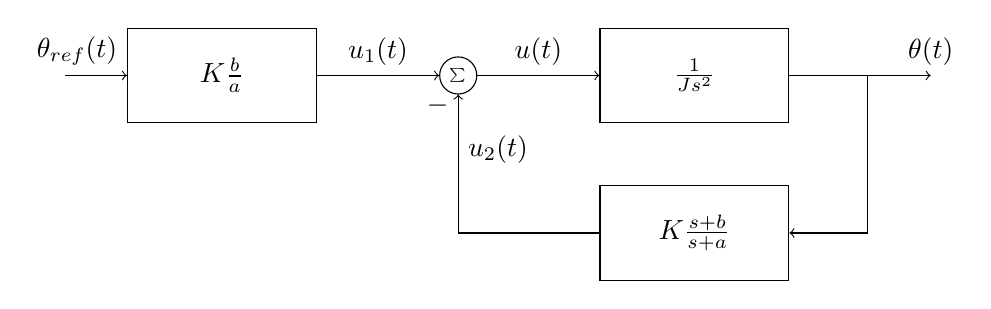
\begin{tikzpicture}
\tikzset{node distance=2cm, 
    block/.style={rectangle, draw, minimum height=12mm, minimum width=24mm},
    sumnode/.style={circle, draw, inner sep=2pt}        
}

  \node[coordinate] (input) {};
  \node[block, right of=input] (TR) {$K\frac{b}{a}$};
  \node[sumnode, right of=TR, node distance=30mm] (sum) {\tiny $\sum$};
  \node[block,right of=sum, node distance=30mm] (plant) {$\frac{1}{Js^2}$};
  %\node[sumnode, right of=plant, node distance=30mm] (sumdist) {$\sum$};
  %\node[coordinate, above of=sumdist, node distance=15mm] (dist) {};
  %\node[coordinate, right of=sumdist, node distance=15mm] (measure) {};
  \node[coordinate, right of=plant, node distance=30mm] (output) {};
  \node[coordinate, right of=plant, node distance=22mm] (measure) {};
  %\node[sumnode,below of=measure, node distance=25mm] (sumnoise) {$\sum$};
  %\node[coordinate, right of=sumnoise, node distance=15mm] (noise) {};
  \node[block,below of=plant, node distance=20mm] (SR) {$K\frac{s+b}{s+a}$};

  \draw[->] (input) -- node[above, pos=0.2] {$\theta_{ref}(t)$} (TR);
  \draw[->] (TR) -- node[above] {$u_1(t)$} (sum);
  \draw[->] (sum) -- node[above] {$u(t)$} (plant);
  \draw[->] (plant) -- node[at end, above] {$\theta(t)$} (output);
  \draw[->] (measure) |- (SR);
  \draw[->] (SR) -| (sum) node[right, pos=0.8] {$u_2(t)$} node[left, pos=0.96] {$-$};
\end{tikzpicture}
\end{center}
\end{frame}
\begin{frame}[label={sec:org15df7f9}]{From continuous-time design to discrete controller}
Let \(y(t)=\theta(t)\). The feedback controller is given in the Laplace-domain as 
\begin{center}
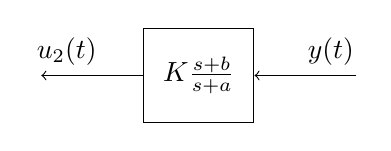
\begin{tikzpicture}
\tikzset{node distance=2cm, 
    block/.style={rectangle, draw, minimum height=12mm, minimum width=14mm},
    sumnode/.style={circle, draw, inner sep=2pt}        
}

  \node[coordinate] (input) {};
  \node[block, left of=input] (SR) {$K\frac{s+b}{s+a}$};
  \node[coordinate, left of=SR] (output) {};
  \draw[->] (input) -- node[above, near start] {$y(t)$} (SR);
  \draw[->] (SR) -- node[above, near end] {$u_2(t)$} (output);
\end{tikzpicture}
\end{center}
\begin{align*}
U_2(s) &= K \frac{s+b}{s+a} Y(s)\\
(s+a)U_2(s) &= K(s+b)Y(s)
\end{align*}
\alert{Activity} Which is the correct corresponding ODE?
\begin{center}
\begin{tabular}{ll}
1: \(\dot{u}_2 + a = K\dot{y} + by\) & 1: \(\dot{u}_2 + a = K\dot{y} + Kby\)\\
3: \(a u_2 + \dot{u}_2 = Kby + K\dot{y}\) & 4: \(a u_2 + \dot{u}_2 = K\dot{y} + by\)\\
\end{tabular}
\end{center}
\end{frame}

\begin{frame}[label={sec:orga251b49}]{Simple discretization}
\begin{center}
\begin{tikzpicture}
\pgfmathsetmacro\tone{2}
\pgfmathsetmacro\ttwo{4}
\pgfmathsetmacro\xone{0.1*\tone*sin(10*\tone)}
\pgfmathsetmacro\xtwo{0.1*\ttwo*sin(10*\ttwo)}
\pgfmathsetmacro\xdot{(\xtwo-\xone)/(\ttwo-\tone)}

\begin{axis}[width=7cm, height=5cm, xtick={\tone, \ttwo}, xticklabels={$t_1$, $t_1+h$},
ytick={\xone, \xtwo}, yticklabels={$x(t_1)$, $x(t_1+h)$}]
\addplot+[no marks, thick, variable=\t, domain = 0:8, samples=100] {0.1*t*sin(10*t)} node[coordinate, pos=0.8, pin=90:{$x(t)$}] {};
\addplot+[ycomb,] coordinates  {(\tone, \xone) (\ttwo, \xtwo)};
\addplot+[this, no marks, variable=\t, domain = -1:3, samples=10] ({\tone + t}, {\xone + \xdot*t});
\end{axis}

\node at (8,3) {\( \dot{x}(t) \approx \frac{\Delta x}{\Delta t} = \frac{x(t + h) - x(t)}{h} \)};
\end{tikzpicture}
\end{center}

Approximating the controller, assuming equidistant sampling  \(t = kh\):
\begin{align*}
a u_2 + \dot{u}_2 &= Kby + K\dot{y}\\
a u_2(kh) + \frac{1}{h} \big(u_2(kh+h) - u_2(kh)\big) &= Kby(kh) + \frac{K}{h}\big(y(kh+h) - y(kh)\big)
\end{align*}
\end{frame}

\begin{frame}[label={sec:org66749d5}]{Simple discretization, contd}
Approximating the controller, assuming equidistant sampling  \(t = kh\):
\begin{align*}
a u_2 + \dot{u}_2 &= Kby + K\dot{y}\\
a u_2(kh) + \frac{1}{h} \big(u_2(kh+h) - u_2(kh)\big) &= Kby(kh) + \frac{K}{h}\big(y(kh+h) - y(kh)\big)
\end{align*}
\[ u_2(kh+h) = (1-ah)u_2(kh) + Ky(kh+h) - K(1-bh)y(kh) \]

This is an algorithm that can easily be implemented on a microcontroller. 
\begin{center}
\includegraphics[width=0.35\linewidth]{../../figures/fig1-7.png} \tiny From Åström and Wittenmark, Computer-controlled systems
\end{center}
\end{frame}


\begin{frame}[label={sec:org2e64ecc}]{Two approaches to designing a  discrete-time controller}
\begin{enumerate}
\item Do design the controller in the continuous-time domain (methods from control engineering class). Then discretize the continuous-time controller.
\includegraphics[width=0.7\linewidth]{../../figures/block1} \(F_d(z) \approx F(s)\)
\item Determine discrete-time model of the plant. Do design in discrete-time domain.
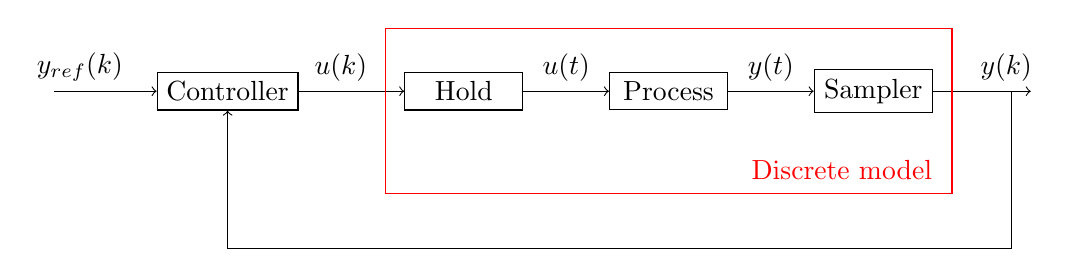
\begin{tikzpicture}[node distance=22mm, block/.style={rectangle, draw, minimum width=15mm}, sumnode/.style={circle, draw, inner sep=2pt}]

  \node[coordinate,] (refinput) {};
  \node[block, right of=refinput] (controller)  {Controller};
  \node[block, right of=controller, node distance=30mm] (zoh)  {Hold};
  \node[block, right of=zoh, node distance=26mm] (plant)  {Process};
  \node[block, right of=plant, node distance=26mm] (sampler)  {Sampler};
  \node[coordinate, right of=sampler, node distance=20mm] (output) {};

  \draw[->] (refinput) -- node[above, near start] {$y_{ref}(k)$} (controller);
  \draw[->] (controller) -- node[above, pos=0.4] {$u(k)$} (zoh);
  \draw[->] (zoh) -- node[above] {$u(t)$} (plant);
  \draw[->] (plant) -- node[above] {$y(t)$} (sampler);
  \draw[->] (sampler) -- node[pos=0.8, coordinate] (measure) {} node[above, near end] {$y(k)$} (output);
  \draw[->] (measure) -- ++(0,-20mm) -| (controller);
  \draw[red] (42mm, -13mm) rectangle (114mm, 8mm);
  \node[red] at (100mm, -10mm) {Discrete model};
\end{tikzpicture}
\end{enumerate}
\end{frame}

\begin{frame}[label={sec:org090c207}]{Discretizing the plant model}
\begin{columns}
\begin{column}{0.3\columnwidth}
\includegraphics[height=0.4\textheight]{../../figures/diskdrive.png}

\tiny "Laptop-hard-drive-exposed" by Evan-Amos - Own work. Licensed under CC BY-SA 3.0 via Commons
\end{column}
\begin{column}{0.7\columnwidth}
\begin{center}
  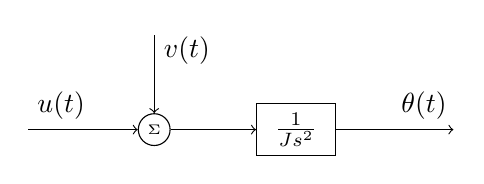
\begin{tikzpicture}[node distance=22mm, block/.style={rectangle, draw, minimum width=10mm}, sumnode/.style={circle, draw, inner sep=2pt}]

    \node[coordinate] (input) {};
    \node[sumnode, right of=input, node distance=16mm] (sum) {\tiny $\Sigma$};
    \node[block, right of=sum, node distance=18mm] (plant)  {$\frac{1}{Js^2}$};
    \node[coordinate, above of=sum, node distance=12mm] (disturbance) {};
    \node[coordinate, right of=plant, node distance=20mm] (output) {};

    \draw[->] (input) -- node[above, pos=0.3] {$u(t)$} (sum);
    \draw[->] (sum) -- node[above] {} (plant);
    \draw[->] (plant) -- node[above, near end] {$\theta(t)$} (output);
    \draw[->] (disturbance) -- node[right, pos=0.2] {$v(t)$} (sum);
  \end{tikzpicture}
\end{center}
\[ J\ddot{\theta}(t) = u(t) + v(t) \]

    \begin{align*} 
      \ddot{\theta}(t) &\approx \frac{ \dot{\theta}(t+h) - \dot{\theta}(t)}{h}\\
                       &\approx \frac{ \frac{ \theta(t+h+h)-\theta(t+h)}{h} - \frac{\theta(t+h)-\theta(t)}{h}}{h}\\
		       &=
\end{align*}

\alert{Activity} Simplify the expression!
\end{column}
\end{columns}
\end{frame}

\begin{frame}[label={sec:orgb83f675}]{Controller design in discrete time}

\begin{center}
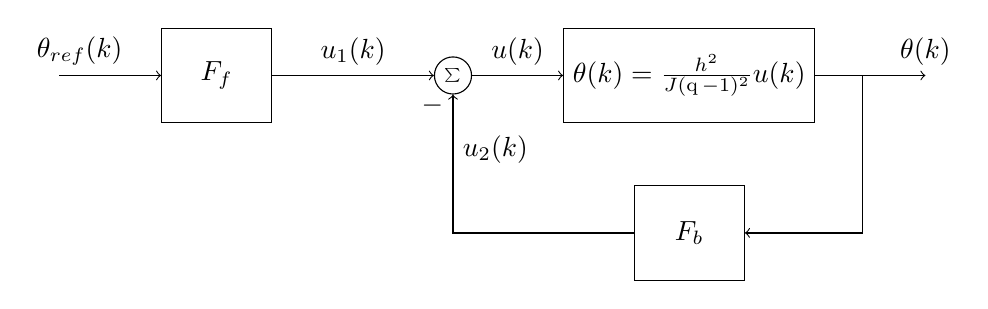
\begin{tikzpicture}
\tikzset{node distance=2cm, 
    block/.style={rectangle, draw, minimum height=12mm, minimum width=14mm},
    sumnode/.style={circle, draw, inner sep=2pt}        
}

  \node[coordinate] (input) {};
  \node[block, right of=input] (TR) {$F_f$};
  \node[sumnode, right of=TR, node distance=30mm] (sum) {\tiny $\sum$};
  \node[block,right of=sum, node distance=30mm] (plant) {$\theta(k) = \frac{h^2}{J(\shift-1)^2}u(k)$};
  %\node[sumnode, right of=plant, node distance=30mm] (sumdist) {$\sum$};
  %\node[coordinate, above of=sumdist, node distance=15mm] (dist) {};
  %\node[coordinate, right of=sumdist, node distance=15mm] (measure) {};
  \node[coordinate, right of=plant, node distance=30mm] (output) {};
  \node[coordinate, right of=plant, node distance=22mm] (measure) {};
  %\node[sumnode,below of=measure, node distance=25mm] (sumnoise) {$\sum$};
  %\node[coordinate, right of=sumnoise, node distance=15mm] (noise) {};
  \node[block,below of=plant, node distance=20mm] (SR) {$F_b$};

  \draw[->] (input) -- node[above, pos=0.2] {$\theta_{ref}(k)$} (TR);
  \draw[->] (TR) -- node[above] {$u_1(k)$} (sum);
  \draw[->] (sum) -- node[above] {$u(k)$} (plant);
  \draw[->] (plant) -- node[at end, above] {$\theta(k)$} (output);
  \draw[->] (measure) |- (SR);
  \draw[->] (SR) -| (sum) node[right, pos=0.8] {$u_2(k)$} node[left, pos=0.96] {$-$};
\end{tikzpicture}
\end{center}

Plant model, using the shift operator \(\shift\) (\(\shift f(k) = f(k+1)\)) and assuming \(h=1\):
\begin{align*}
\theta(k+2) - 2\theta(k+1) + \theta(k) &= \frac{h^2}{J} u(k)\\ 
\shift^2 \theta(k) - 2\shift \theta(k) + \theta(k) &= \frac{h^2}{J} u(k)\\
(\shift^2 - 2\shift + 1) \theta(k) &= \frac{h^2}{J} u(k)
\end{align*}
\end{frame}


\begin{frame}[label={sec:org0896390}]{Discretizing analog design will be worse than the analog performance}
\begin{center}
\includegraphics[width=0.7\linewidth]{../../figures/fig1-8.png}
\end{center}
\end{frame}

\begin{frame}[label={sec:org64f2e99}]{Discrete design can give better performance}
\includegraphics[height=0.6\linewidth]{../../figures/fig1-9.png}
\end{frame}

\begin{frame}[label={sec:orga573ae3}]{Challenges with computerized control - aliasing}
\begin{columns}
\begin{column}{0.6\columnwidth}
\begin{center}
  \begin{tikzpicture}
    \node {\includegraphics[width=0.99\linewidth]{../../figures/comp-contr-sys.png}};
    \node[pin=145:{60Hz mains hum}] at (2.7,2.4) {};
    \node[pin=-60:{90Hz sampling freq}] at (0.5,-1.4) {};
  \end{tikzpicture}
\end{center}
\end{column}
\begin{column}{0.4\columnwidth}
\includegraphics[width=0.99\linewidth]{./aliasing-example-60Hz}
\end{column}
\end{columns}
\end{frame}


\begin{frame}[label={sec:org8f7af18}]{Challenges with computerized control - aliasing}
\begin{block}{Aliasing}
\includegraphics[height=0.6\textheight]{../../figures/Moire_pattern_of_bricks.png} \hspace*{3mm} \includegraphics[height=0.6\textheight]{../../figures/Moire_pattern_of_bricks_small.png}
{\tiny From wikipedia, Creative Commons}

\alert{Sampling can create frequencies that do not exist in the real signal}
\end{block}
\end{frame}

\begin{frame}[label={sec:org66cb20f}]{Challenges with computerized control}
\begin{block}{Sampling causes a delay of approximately half the sampling period}
\includegraphics[width=0.9\textwidth]{../../figures/modulation-model-timeseries}
\end{block}
\end{frame}


\begin{frame}[label={sec:orgf3ad391}]{Why computerized control?}
\begin{itemize}
\item Almost all control systems are implemented on computers/microcontrollers/PLCs
\item Controllers designed in continuous-time must be discretized to be implemented on a computer - What does this mean for the performance?
\item Design that takes into account the discrete nature of the computer can give better performance
\end{itemize}
\end{frame}

\section{Course content structure}
\label{sec:org754a567}

\begin{frame}[label={sec:org1e8c60c}]{Course book}
\begin{center}
\includegraphics[width=0.4\linewidth]{../../figures/tec-book.png}
\end{center}
\end{frame}

\section{Course structure}
\label{sec:org6e9a9f3}
\begin{frame}[label={sec:orgfd160b4}]{Homework}
\begin{itemize}
\item Every week
\item Solved in groups of 3, handed in on Canvas
\item Each homework accounts for 7\% of final grade
\end{itemize}
\end{frame}

\begin{frame}[label={sec:org890336d}]{Examination and grading}
\begin{itemize}
\item Homework 35\%
\item Partial exam 1 20\%
\item Partial exam 2 20\%
\item Final exam 25\%

Each exam consists of quiz on Canvas (50\%) and video assignment (50\%)
\end{itemize}
\end{frame}
\end{document}